\chapter*{Introduction}
\graphicspath{{fig/}}
\chaptermark{Introduction}
\markboth{\MakeUppercase{Introduction}}{}
\addcontentsline{toc}{chapter}{Introduction}
\section*{Turbulent flows}
\addcontentsline{toc}{section}{Turbulent flows}
Everybody has most probably heard of the word turbulence. It has its origin
from the Latin word \emph{turba} and refers to the disorderly motion of a
crowd. In the middle ages it was frequently used as a synonym for ``trouble''.
Nowadays, this ``trouble'' is still acknowledged not only by engineers and
scientists, but also by tourists on a flight, as an aircraft will
literally shake when it enters a zone of turbulence.  In general, the word
turbulence is used to indicate irregularities, fluctuations, and sometimes
even chaos.  While this can apply to many topics like politics  in times of
conflict of a government (political turbulence), in this dissertation we imply
the fluid dynamical meaning of the word turbulence.
While most scientists agree on what a turbulent flow is, they find it
difficult to define an exact definition for the problem. It is therefore
generally defined by typical characteristics such as randomness,
non-linearity, enhanced diffusivity, vorticity, and dissipation
\citep{Kundu2008}.  To determine the level of turbulence, the so-called
Reynolds number is used which is defined as the ratio of inertial to viscous
forces.  For macroscopic flows that are generally encountered in everyday
life, the Reynolds number is much larger than unity, and therefore these flows
are almost always turbulent.
Many of these flows are hidden as these flows, such as for example air, are not
visible to the human eye.
Simply moving your hand through
the air will create an incalculably complex motions of fluid.  However, when
paying a bit of attention, we can see the turbulence mixes the milk in our
coffee, see the difference in density when hot air is rising above the street
on sunny day, or by observing the flame from a candle. While not directly
visible, turbulence is also seen in our Sun, in the clouds of Jupiter, and
even in our arteries. One of the major difficulties in describing turbulence
resides in the many characteristic length and time scales of the flow. Energy
enters the system in large swirls or eddies, which ``feed'' their energy to
smaller eddies. This already fascinated Leonardo da Vinci, who, as one of
the first, studied turbulent flows in the early 1500s (see
figure \ref{fig:intro_davinci}). In this figure, Leonardo illustrates the many
different length scales which are merely visible on the interface of the fluid
surface.
\begin{figure}[h]
    \centering
    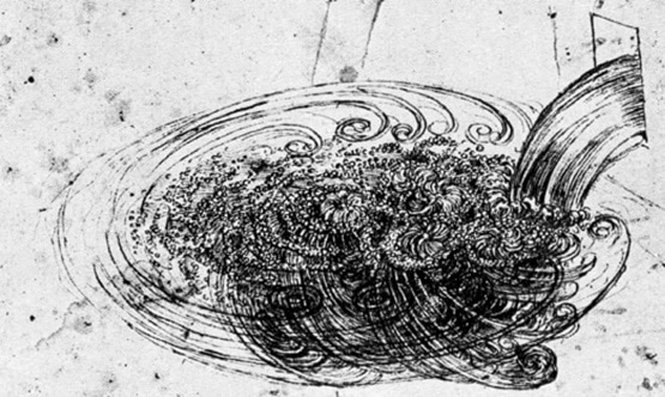
\includegraphics[width=0.8\linewidth]{DaVinci1508.jpg}
    \caption{In the years between 1508 and 1513, Leonardo da Vinci illustrated
    the flow patterns produced by a water yet entering a larger vessel. The
illustration depicts various sizes of eddies, typical for turbulent flows.
\textit{Source: Leonardo da Vinci (RL 12660, Windsor, Royal Library)}}
    \label{fig:intro_davinci}
\end{figure}

When applying Newton's second law of motion, $F=m a$, to a fluid with regular
material properties, \textit{i.e.} a Newtonian fluid such as water, the
governing equations of a turbulent flow can be deducted.  While these,
so-called Navier-Stokes equations (NS) are known for a relatively long time,
it is yet one of the unsolved problems in physics. The problem lies in the
non-linear nature of these equations and they can only be solved analytically
for a couple of special cases. Therefore, to increase the understanding of
turbulent flows we are still highly dependent on simulations and particulary
laboratory experiments. 
\newpage
\section*{Multiphase flows}
\addcontentsline{toc}{section}{Multiphase flows}
Most flows occurring in nature or industrial applications do not consist of a
single phase, but contain inclusions like particles, other (immiscible)
fluids, or a gaseous phase. Examples of such flows are the transportation of
pollen in the air, the transport of sediment in rivers, or the production of
emulsions in the food industry. These bubbles, droplets, or particles are
influenced by the underlying complex turbulent flow structures, and in
response, the flow is itself also influenced by the inclusions. These
interactions are far from trivial and complicate the problem of turbulence
even further. The various physical mechanisms that occur in multiphase flows,
such as particle collisions, bubble break-up, and droplet merging, lack a
unifying view when it comes to theoretical descriptions. Experimentally, it is
possible to measure global properties, such as torque very accurately.
However, to get a better understanding of the underlying physics, also local
quantities, such as droplet size are required. In experiments, it is difficult
to get these local quantities as the different inclusions generally block the
optical pathway for optical measurement techniques. This limits the
non-invasive optical techniques to measure only very close to the boundary of
the system. A way to overcome this is using a probe to measure inside the
flow, however this probe will have an effect on the flow and thereby,
introduce a bias to the measurements itself.  With the increase in computing
power, simulations on turbulent flows become more and more accessible and the
gap between experiments and simulation is closing.  One challenge for
turbulent simulations in general is that all length scales in the system need
to be resolved, from the largest energy input scales to the smallest
dissipation scales. Currently, a few to multiple thousands of particles can be
simulated in numerous flow geometries, including simulations of deformable
droplets\citep{Spandan2018}. The major benefit for using simulations is that
all flow variables, including the local quantities, are available.
Unfortunately, adding inclusions will increase the complexity of these
simulations tremendously, and therefore, limiting the Reynolds numbers
possible to be simulated. Another difficulty lays in simulating dynamic
processes such as coalescence and breakup of droplets as these can currently
only be modelled. These severe limitations of the numerical tools can become
very restrictive in simulating large scale systems that are relevant in
industrial applications and fundamental research.
\newpage
\section*{Roughness and drag reduction}
\addcontentsline{toc}{section}{Drag reduction}
In the last fifty years, the field of turbulent drag reduction has received a serious
amount of attention, especially from the maritime industry. With a projected
consumption of 500 million tonnes per year of heavy fuel oil in 2020
\citep{tradefuel2009}, reducing this amount only with a few percent would
already result in tremendous financial savings. As these types of fuel contain
much higher sulphur levels than diesel, also the environment would greatly
benefit from these drag reductions. Drag on maritime vessels is categorized in
three components: pressure drag, residual drag, and skin friction. The
pressure drag component is directly connected to the submerged geometry of the
ship. Residual drag originates from the generation of bow and stern waves as
seen in figure \ref{fig:intro_wave}. To reduce these types of waves and
thereby, reducing the energetic losses, a so-called \emph{bulbous bow} is
added just below the front waterline of large vessels. These are designed such
that the waves generated by the bulb and bow cancel each other out. Skin
friction drag is in general the largest component of drag which can account
for up to \SI{90}{\percent} of the total drag experienced by the vessel
\citep{Schultz2010}.
\begin{figure}[h]
    \centering
    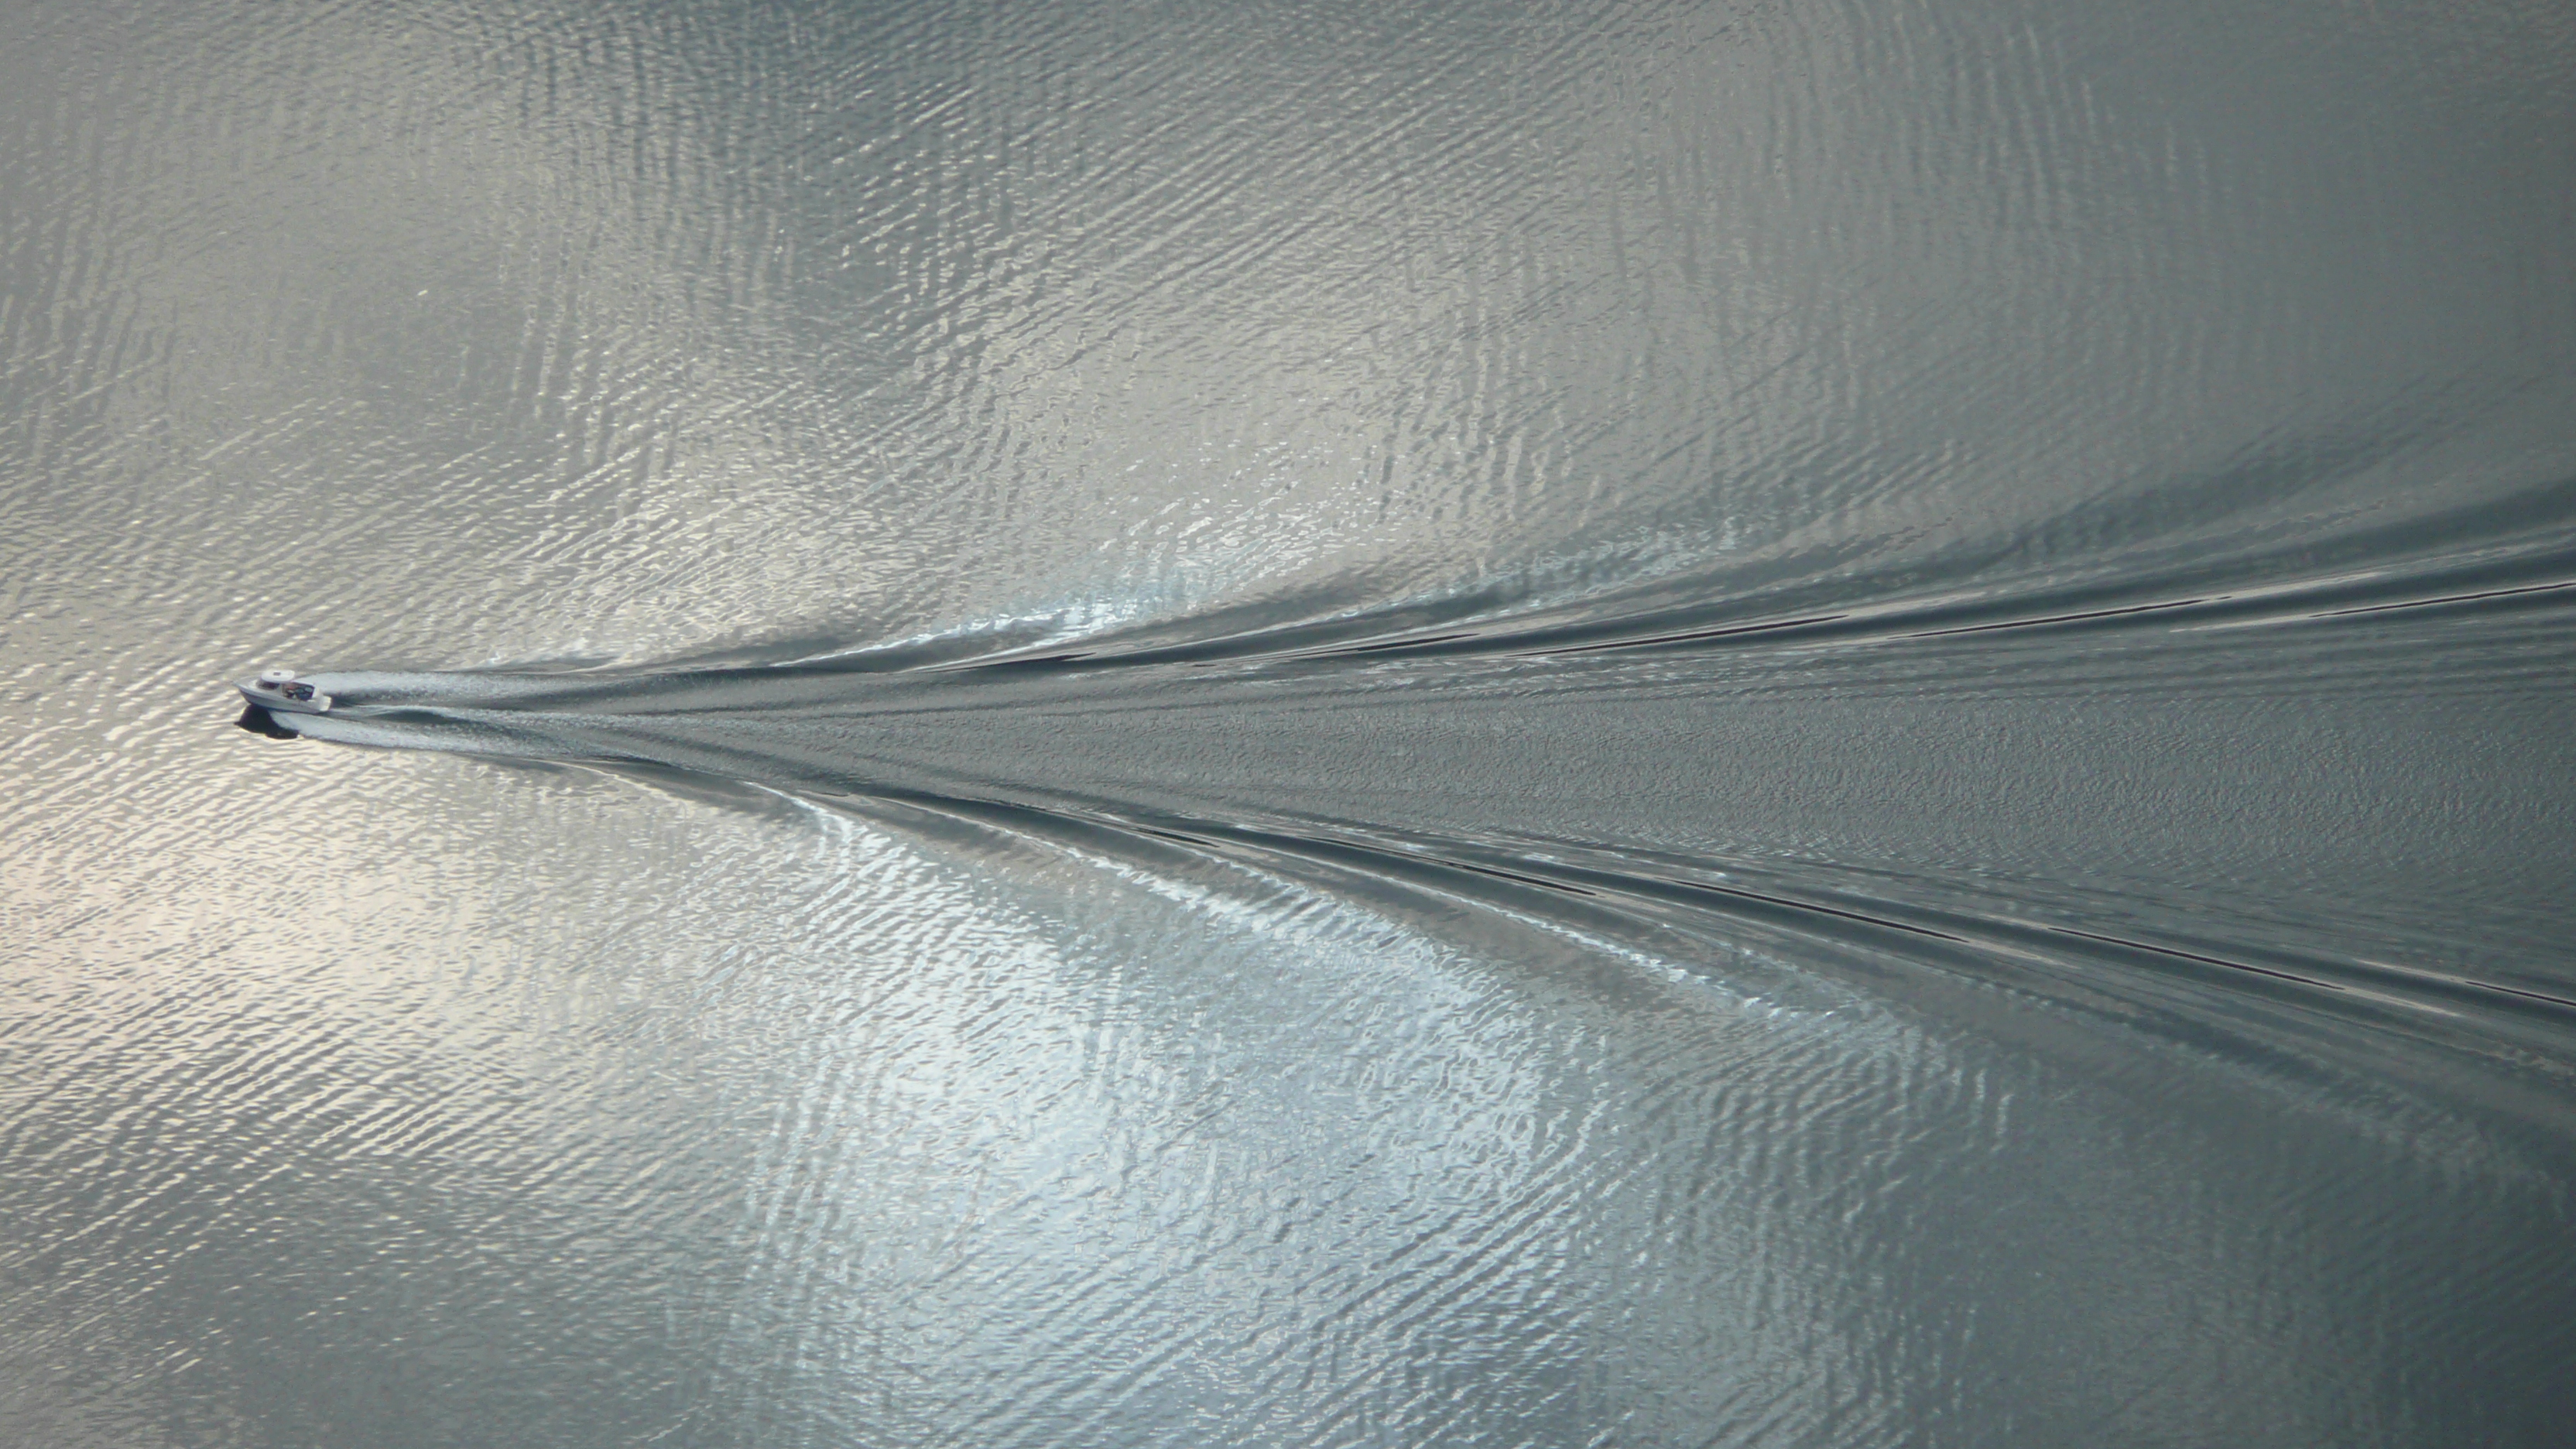
\includegraphics[width=0.8\linewidth]{fig/wakepattern.jpg}
    \caption{Boat sailing the Lyse fjord in Norway. The small vessel
    generates waves on the water surface, thereby, losing energy in the form
    of residual drag. \textit{Photograph: Edmont (Wikipedia.org)}}
    \label{fig:intro_wave}
\end{figure}
It is caused by the viscous drag in the boundary layer of the ship's hull 
for example highly dependent on the surface morphology of the wetted area. Not
only do, for example, oysters, bacteria, and biofilms increase the degree of
roughness of the ship's hull, but when the Reynolds number (\textit{i.e.}
velocity of the ship) is sufficiently large, even a seemingly smooth surface
becomes hydrodynamically rough. One way to cut down these frictional losses is
to introduce an air layer on the ship's hull \citep{Verschoof2018b}. This
layer acts as a lubrication layer between the water and the hull, reducing the
wetted area. One of the first laboratory experiments created micro bubbles
using electrolysis below a scale model \citep{mcCormick1973} and found
reductions of up to \SI{30}{\percent}. Now, almost fifty years later, the
underlying physics of the drag reduction are still not well understood and the
key parameters are still not known.  It is difficult to isolate parameters
such as size, deformability, and shape, which can all be important for the
process.  While currently there are commercial products available, full scale
experiments show an almost unpredictable rate of success. There are as many
reports on reduction in drag, as there are cases reporting a drag
increase\,\cite{Murai2014}. It
is not always clear if these studies report \emph{net} drag reduction,
\textit{i.e.} take into account the additional energy required to inject air.
All these uncertainties result in that the current, rather expensive
technology is yet not applied to current maritime vessels. 

\section*{Taylor-Couette flow and Rayleigh-B\'enard convection}
\addcontentsline{toc}{section}{Taylor-Couette flow and Rayleigh-B\'enard convection}
Taylor-Couette flow (TC) and Rayleigh-B\'enard convection (RB) are 
canonical systems in physics of fluids, and have already been called the
``twins of turbulence research'' \citep{Busse2012}. This is because both
systems are mathematically well-defined and they have exact energy balances
between global energy input and dissipation.

In a Taylor-Couette geometry, the fluid is confined between two independently
rotating concentric cylinders. These types of flows got a tremendous amount of
attention in the past two decades \citep{Grossmann2016}. A schematic
of a typical setup is shown in figure \ref{fig:intro_setup}a. The inner and
outer cylinders have radii $r_i$ and $r_o$, respectively, and both cylinders
can rotate independently with angular velocities $\omega_i$ and $\omega_o$.
The gap size between the two cylinders is $d=r_o-r_i$ and the total height of
the cylinder is $L$. These measures can be combined to get the geometric
parameters of the system: the aspect ratio $\Gamma=L/d$ and the radius ratio
$\eta=r_i/r_o$.  The complete control parameters of this system consists of
these geometric parameter, together with two Reynolds number,
$\text{Re}_{i,o}=\omega_{i,o} r_{i,o} d / \nu$, where the subscripts denote
the inner or outer cylinder quantities and $\nu$ is the kinematic viscosity.
The primary response of the system is the torque $\tau$ required to maintain
the cylinders at constant speed. Typically, this torque is non-dimensionalized
to the dimensionless torque $G=\tau / (2 \pi L \rho \nu^2)$ or the friction
coefficient $C_f=\tau / (L\rho\nu^2(\text{Re}_i - \eta\text{Re}_o)^2)$, where
$\rho$ is the density of the fluid. In simulations, the local flow properties
are accessible as the complete flow structure is known, however, the Reynolds
numbers is still relatively limited, especially for multiphase flows.
Therefore, to study these local flow properties we still heavily rely on
laboratory measurements. Examples of such measurements are laser Doppler
anemometry (LDA) and particle image velocimetry (PIV), which are both
non-intrusive measurements but require optical access to the measurement area
(see figure \ref{fig:intro_setup}a).

\begin{figure}[ht]
    \centering
    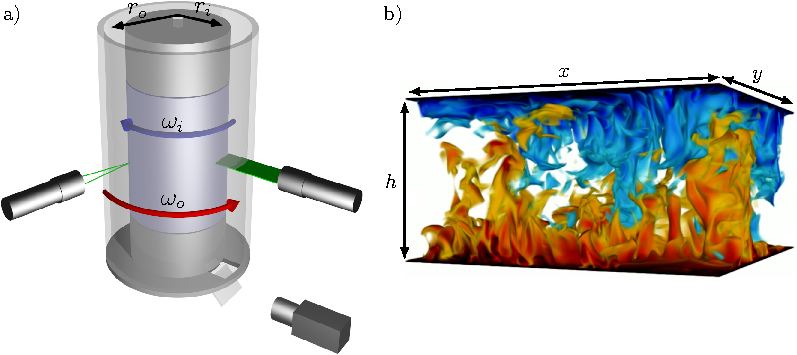
\includegraphics[width=1.0\linewidth]{fig/setup/setup.pdf}
    \caption{a) A schematic of a Taylor-Couette apparatus. The
    flow is confined between two concentric cylinders that can rotate
    independently. Torque is measured at the middle segmented cylinder
    (highlighted in diagram). The transparent outer cylinder makes it possible
    to access the flow using non-intrusive measurement techniques like LDA and PIV. b)
    Instantaneous temperature field from direct numerical simulations of a
    Rayleigh-B\'enard convection cell. Only hot (red) and cold (blue) fluid is
    visualized to identify the plume structures. \textit{(DNS snapshot courtesy
    of Erwin P. van der Poel)}.}
    \label{fig:intro_setup}
\end{figure}

For Rayleigh-B\'enard convection, the flow is heated from below and cooled
form the top\citep{Lohse2010}. A typical instantaneous temperature snapshot from direct
numerical simulations (DNS) is shown in figure \ref{fig:intro_setup}b
(courtesy Erwin~P.~van~der~Poel). The top and bottom plates are separated by a
distance $h$ and have a temperature difference $\Delta$. The driving parameter of
the system is the Rayleigh number $\text{Ra}=\beta g \Delta h^3 / (\kappa
\nu)$, where $\beta$ is the thermal expansion coefficient, $g$ the
acceleration due to gravity, and $\kappa$ the thermal diffusivity.  A
three-dimensional system has two aspect ratios, $\Gamma_x=x/h$ and
$\Gamma_y=y/h$, for each horizontal dimension. In simulations it is common to
express the fluid in form of a Prandtl number $\text{Pr}=\nu/\kappa$. The
response of the system, after setting the control parameters $\Gamma_x$,
$\Gamma_y$, $\text{Pr}$, and $\text{Ra}$, is the heat transport which is
quantified by the Nusselt number $\text{Nu}=J/J_c$, where $J$ is the heat
flux from the bottom to the top plate and $J_c$ is the pure conductive
component.

TC flow and RB convection are mathematically very similar \citep{Eckhardt2006}
and have conserved quantities: angular velocity flux in TC and heat flux in
RB. Using this analogy, the quantities in TC can be rewritten in terms that
resemble RB \citep{Eckhardt2007}. The driving and response of TC can be
expressed as the Taylor number and a ``$\omega$--Nusselt number'' for TC:
\begin{align}
\text{Ta}&=\frac{1}{4}\left(\frac{1+\eta}{2\sqrt{\eta}}\right)^4(r_o - r_i)^2
(r_i + r_o)^2(\omega_i - \omega_o)^2/\nu^2\\
\text{Nu}_\omega&=\frac{J_\omega}{J_{\omega,\text{lam}}}
\end{align}
here, $J_\omega$ is the angular velocity flux from the inner to the outer
cylinder and $J_{\omega,\text{lam}}$ is the laminar flow contribution. By
using these terms, the transport quantity scales as a function of the driving
parameter with a certain scaling exponent $\gamma$, analogous to RB.

\section*{Outline of the thesis}
\addcontentsline{toc}{section}{Outline of the thesis}
This thesis can be divided in two main topics: turbulent flows with inclusions
and the interaction of patterned roughness on large flow structures.
A flow holding inclusions can increase or decrease the skin friction at the
boundary, \textit{e.g.} a ship's hull or the wall of a pipeline.
The inclusions itself have many parameters like size, shape, and
deformability.
We however, are lacking the understanding how these parameters
influence the skin friction.
In \refc{chap:spheres}, by using solid neutrally buoyant spherical
particles we disentangle three of these effects: size, deformability, and
particle volume fraction.
The drag of a rotating inner cylinder is measured while varying the size and
the amount of these particles, and afterwards thoroughly compared to results
from bubbly drag reduction.
In \refc{chap:fibers} the shape of the particle is changed to an elongated
cylinder and therefore, the orientation of a particle becomes important.
Using high-speed imaging, we track the translation and orientation
of the particles and investigate any collective effects.
Chapter\,\ref{chap:emulsions} presents the work on meta-stable emulsions in a
turbulent flow.
By applying intense shear, an immiscible fluid is suspended into another
and therefore, creating deformable inclusions if the droplets are large.
Exploiting the scaling of the momentum transfer in the ultimate regime of
Taylor--Couette flow, it is possible to calculate an effective viscosity for
the mixture.
We answer how the morphology of the emulsion and the droplet size connects to
the measured friction of the system.
In \refc{chap:mixedbc}, using direct numerical simulations, we investigated the effect of 
non-homogeneous driving of a Rayleigh-B\'enard cell.
The top or both plates were divided in a stripe or checkerboard pattern,
which consisted of alternating insulating or conducting temperature boundary
conditions.
While varying the periodic pattern using a wave number we have studied global
quantities such as the effective heat transfer.
Using a Fourier transform, it is possible to see the imprint of the pattern
and study the penetration depth of such boundary conditions.
In the same spirit as \refc{chap:mixedbc}, in \refc{chap:spanwise} we applied
spanwise roughness to the driving cylinder of the Taylor--Couette setup,
thereby, also having non-homogeneous driving of the flow.
Using laser Doppler anemometry, it is possible to study the imprint of
the pattern in the bulk flow.
Using particle image velocimetry and torque measurements, we can investigate
how the secondary flows, \text{i.e.} the turbulent Taylor vorices, are
influenced by the spanwise roughness and how these are linked to the global
transport.
Finally, we conclude and summarize the work done is this thesis.

